\documentclass[12pt,a4paper]{article}
\usepackage[utf8]{inputenc}
\usepackage{amsmath}
\usepackage{amssymb}
\usepackage{placeins}
\usepackage{amsthm}
\usepackage{amsfonts}
\usepackage{graphicx}
\usepackage[all]{xy}
\usepackage{tikz}
\usepackage{verbatim}
\usepackage{float}
\usepackage{bbm} %indicator function 1 package
\usepackage{bbold} %indicator function 1 package with bold
\usepackage[left=2cm,right=2cm,top=3cm,bottom=2.5cm]{geometry}
\usepackage{hyperref}
\usepackage{caption}
\usepackage{subcaption}
\usepackage{psfrag}
\usepackage{mathrsfs}
\author{Yusuf Brima}
\title{Towards understanding Potential Evapotranspiration across 10 African cities using Statistical Machine Learning}
\begin{document}
\maketitle
\thispagestyle{empty}
\pagebreak
\begin{abstract}
The world is rapidly evolving at an unprecedented rate largely due to human actions on the environment. The effects of  this  change is being noticed through variable patterns in the climate across the global which is projected to have unforeseen consequences in the near and far future. Climate change is a prevailing threat existential crisis we are facing as a human species which if not mitigated will have devastating consequences on us and our surrendering fauna and flora. Therefore,  in this work,  we use state-of-the-art Hierarchical Cluster Analysis (CA) and Principal Component Analysis (PCA) algorithms. We found four clusters for the 10 cities with similar Potential Evapotranspiration and using PCA (both non rotated and rotated) to identify the underlying processes that gave rise to the factors of variation int the data set wherein we identified two principal components using varimax that explain nearly 90 per cent of variability in the data. 
\end{abstract}
\pagenumbering{roman}
\pagebreak
\tableofcontents
\pagebreak
\section{Introduction}
\pagenumbering{arabic}
Climate change is one of the prevailing threats existential crisis we are facing as a human species which if not mitigated will have devastating consequences on us and our surrendering fauna and flora. This effect is large since the climatic condition of the atmosphere dictates the survival ability of all life forms, the civilization we take for granted is hinged on our ability to produce food on an industrial scale to cater for the soaring global population, availability of clean air and freshwater systems as well as the ozone layer of the atmosphere to shield us from ultraviolet radio from the sun.
A scholarly exposition of the effect of climatic changes is crucial for especially the developing world where the effect of such changes is projected to have greater impact leading to extreme events such as droughts, flooding,  hurricanes, famines, the rise of sea levels along coastal regions.  These events starkly have the potential to undermine economic activities and political stability.
\section{Research Problem}
Understanding the effect of evapotranspiration patterns across different geographic regions across the African continent is pivotal to coordinated climate action and policy formulation. However, this process involves aggregating big data sets from locations that have varied underlying factors of variation in the processes that generated the data. 
\section{Research Objective}
\begin{enumerate}
\item[(I)] The object of this research is to explore the characteristics of three Cluster Analysis (CA) algorithms using the provided climate dataset over African cities (Kamembe, Kayonza, Kigali, Koulikoro, Lagos, Lome, Maseno, Mombasa, Musanze, Nairobi ) using evapotranspiration.  
This is done to show the sensitivity of the grouping to three Cluster Analysis algorithms (single linkage, average linkage,  and Ward’s algorithm) and make a comparative analysis the results as well as the physical interpretation of those findings.
\item[(II)] The second object of this work is to study the characteristics of Principal Component Analysis (PCA) algorithm and contrast it with that of CA using the data set in question from ten African cities using evapotranspiration.  We seek to explore the sensitivity
of PCA analysis to (i) rotated and (ii) non-rotated PCA methods and the temporal variation of the  Principal Factors (PFs) over the study period.  Finally,  we give physical interpretations of our findings in comparison with the objective I.
\end{enumerate}
\section{Research Methodology}
\subsection{Evapotranspiration}
Potential Evapotranspiration (PET) is the sum of water evaporation and transpiration from a surface area to the atmosphere.  Evaporation accounts for the movement of water to the air from sources such as the soil, canopy interception, and water bodies as depicted in Figure \ref{fig:evapo}.
\begin{figure}[!h]
			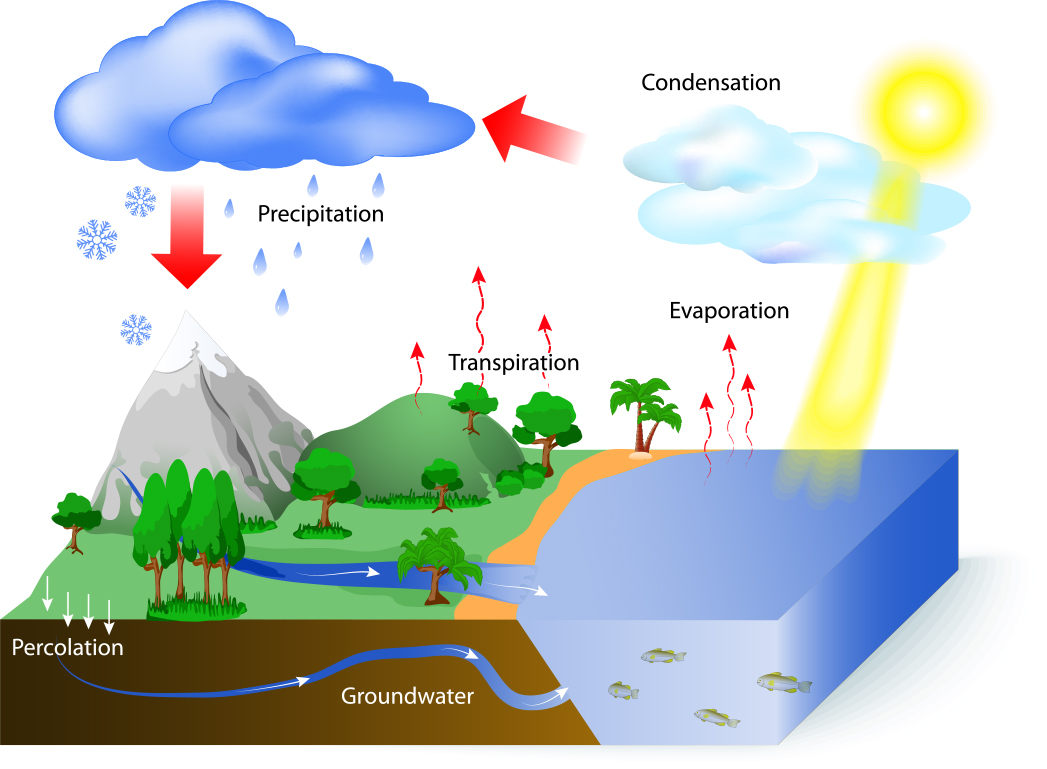
\includegraphics[width=430pt,  height=215pt]{./gaphics/evapotranspiration.jpg}
			\caption{Illustration of Evapotranspiration}
			\label{fig:evapo}
\end{figure}
\subsection{Research Instruments}
In this research, we use Cluster Analysis technique to group ten African cities (Kamembe, Kayonza, Kigali, Koulikoro, Lagos, Lome, Maseno, Mombasa, Musanze, Nairobi ) based on their evapotranspiration patterns.
The CA algorithm explores three different linkage methods viz: single linkage,  average linkage,  and Ward’s algorithm to investigate their effect on the cluster formation of clustering parameters.

We further subject the same dataset to PCA algorithm with a goal of understanding the principal factors of variation that impact the evapotranspiration process for the cities in being studied with  sensitivity
of PCA analysis to (i) rotated and (ii) non-rotated PCA.

The primary computational tool for our experiment is the R programming language primarily because it is well suited and expressive to undertake high-level rapid exploratory data analysis for scientific reporting as well as being able to automate repetitive predictive analytic processes which all aid reproducibility of research.
\subsection{Data set}
We utilise a secondary data set of evapotranspiration in this report from ten African cities (Kamembe,  Kayonza,  Kigali,  Koulikoro,  Lagos,  Lome,  Maseno,  Mombasa,  Musanze,  Nairobi ) with different geographic conditions.  This consists of 10 parameters (i.e.,   evapotranspiration for each city) and 612 observations (monthly averaged evapotranspiration ) from January 1960 to December 2010 (50 years).
\pagebreak
\section{Results and Discussions}
\subsection{Results}
In this section of report, we present the empirical observations after carrying out CA and PCA on the Potential Evapotranspiration data set for the ten cities being studied.
\subsubsection{Cluster Analysis}
\begin{figure}[!h]
    \centering
    \begin{subfigure}[t]{0.3\textwidth}
        \centering
        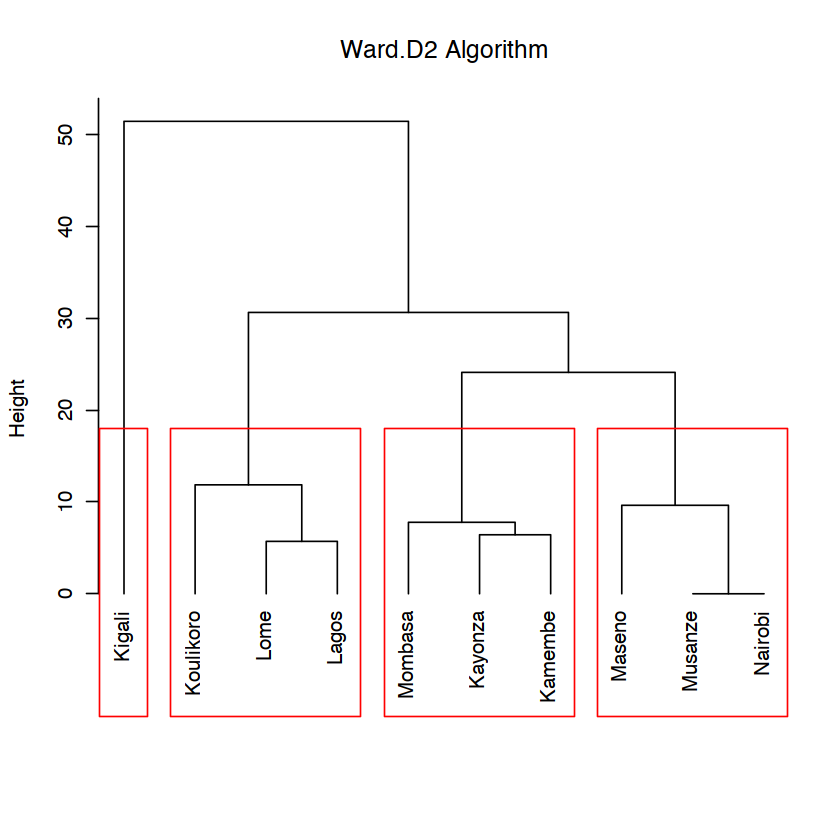
\includegraphics[height=1.8in]{./gaphics/q001_a.png}
        \caption{}
    \end{subfigure}%
    ~ 
    \begin{subfigure}[t]{0.3\textwidth}
        \centering
        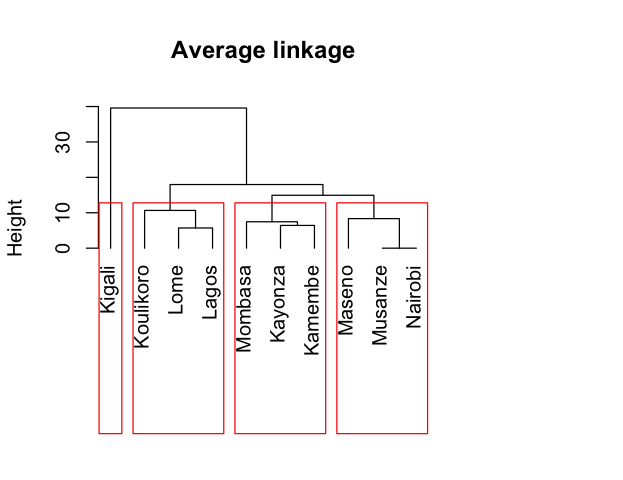
\includegraphics[height=1.8in]{./gaphics/q001_b.png}
        \caption{}
    \end{subfigure}%
    ~ 
    \begin{subfigure}[t]{0.3\textwidth}
        \centering
        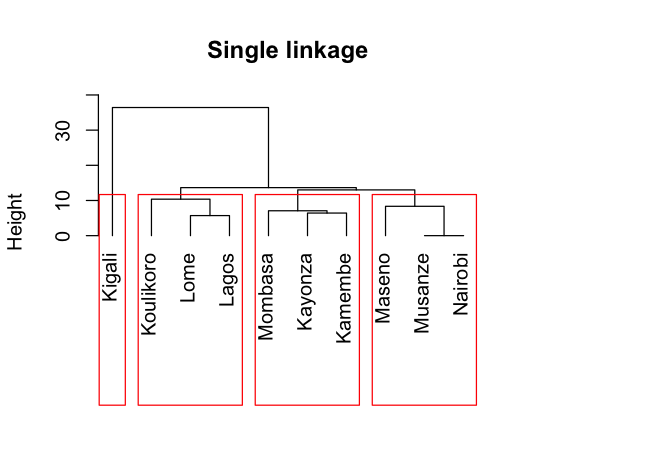
\includegraphics[height=1.8in]{./gaphics/q001_c.png}
        \caption{}
    \end{subfigure}
    \label{fig:cluster_algorithms}
    \caption{Cluster Analysis with 3 distinct linkage algorithms}
\end{figure}
The dendogram in Figure 2 presents the impact of using Ward.D2,  Average and Single linkage algorithms on the data set using a cluster value (K = 4). The red rectangle in the sub figures indicate cities that belong to the same evapotranspiration grouping thereby resulting on four clusters for the 10 cities in each on the linkage algorithms.
\begin{figure}[!h]
	  \centering
        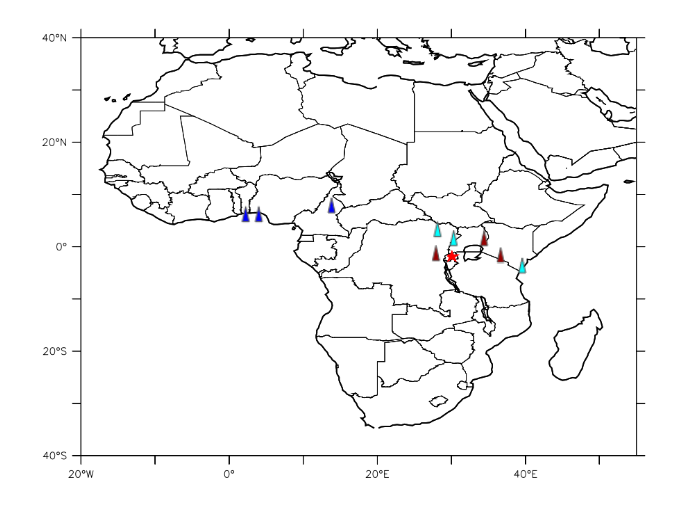
\includegraphics[height=2.4in]{./gaphics/cluster_map.png}
        \caption{Map representation of the clustered cities}
        \label{fig:cluster_map}
\end{figure}

In Figure \ref{fig:cluster_map}, we overlay the Ward.D2 cluster result onto the coordinates (longitude and latitude) of the 10 cities to infer physical and geographical interpretation of the results.  Such visual representation of the clustered data gives rise to rich geographical interpretation for the trend of Potential Evapotranspiration in the cities being studied.
\subsubsection{Principal Component Analysis}
PCA is one of the popular dimensionality reduction alogrithms,  it extracts fewer and independent underlying factors of variation around which the data variance is organised.  This is achieved by identifying principal processes that explain the largest variability in the data set. 
Therefore, in this study, our principal motivation for factor analysis using PCA is to understand the underlying principal processes that drive Potential Evapotranspiration across the ten cities. The Figures (a) and (b) below indicate the screeplot of the eigenvalues and the Percentage Variance Explained (PVE) of the ten principal components using varimax rotation.
From Figures (a) and (b),  clearly indicate that the first and second principal components explain nearly 90 per cent of the variability in  the underlying processes that generated the data.
\begin{figure*}[!h]
    \centering
    \begin{subfigure}[t]{0.5\textwidth}
        \centering
        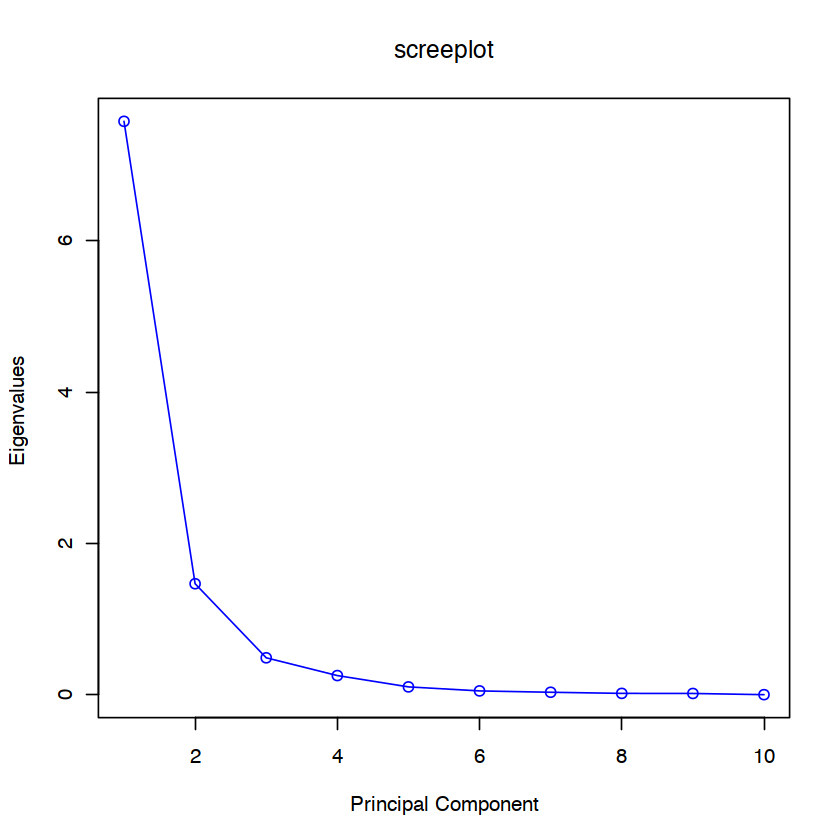
\includegraphics[height=1.9in]{./gaphics/q002_b.png}
        \caption{}
    \end{subfigure}%
    ~ 
    \begin{subfigure}[t]{0.5\textwidth}
        \centering
        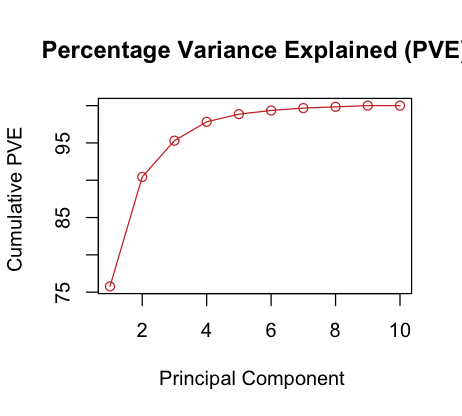
\includegraphics[height=1.9in]{./gaphics/q002_c.png}
        \caption{}
    \end{subfigure}
    \caption{Principal Component Analysis}
\end{figure*}
To further understand the effect of the underlying processes of the principal components, we have plotted a 10 year window time series for the two rotations in the figure below.

\textbf{PCA Loadings (unrotated)}
\begin{verbatim}
Loadings:
          PC1    PC2    PC3    PC4    PC5    PC6    PC7    PC8    PC9    PC10  
Musanze    0.912  0.309 -0.241                                                 
Mombasa    0.899  0.211  0.348 -0.109                                          
Maseno     0.856  0.342 -0.333         0.143 -0.129                            
Lome       0.901 -0.321         0.255                                          
Lagos      0.882 -0.361         0.272                                          
Koulikoro  0.907 -0.343                0.195  0.132                            
Kigali    -0.360  0.862  0.244  0.246                                          
Kayonza    0.952  0.131  0.170 -0.153               -0.117                     
Kamembe    0.961         0.200 -0.126                       0.103              
Nairobi    0.912  0.309 -0.241                                                 

                 PC1   PC2   PC3   PC4   PC5   PC6   PC7   PC8   PC9 PC10
SS loadings    7.578 1.466 0.487 0.252 0.103 0.050 0.032 0.017 0.016    0
Proportion Var 0.758 0.147 0.049 0.025 0.010 0.005 0.003 0.002 0.002    0
Cumulative Var 0.758 0.904 0.953 0.978 0.989 0.994 0.997 0.998 1.000    1
\end{verbatim}

\textbf{PCA Loadings (unrotated)}
\begin{verbatim}
Loadings:
          RC3    RC1    RC4    RC2    RC5    RC7    RC6    RC9    RC8    RC10  
Musanze    0.866  0.400  0.272               -0.110                            
Mombasa    0.443  0.830  0.328                                                 
Maseno     0.899  0.301  0.233                0.200                            
Lome       0.378  0.397  0.750  0.352                       0.112              
Lagos      0.333  0.380  0.777  0.358                                          
Koulikoro  0.389  0.481  0.534  0.478  0.323                                   
Kigali                  -0.242 -0.970                                          
Kayonza    0.547  0.737  0.322  0.132                0.162                     
Kamembe    0.504  0.748  0.373  0.178                              0.119       
Nairobi    0.866  0.400  0.272               -0.110                            

                 RC3   RC1   RC4   RC2   RC5   RC7   RC6   RC9   RC8 RC10
SS loadings    3.463 2.736 2.061 1.479 0.121 0.066 0.034 0.022 0.018    0
Proportion Var 0.346 0.274 0.206 0.148 0.012 0.007 0.003 0.002 0.002    0
Cumulative Var 0.346 0.620 0.826 0.974 0.986 0.993 0.996 0.998 1.000    1
\end{verbatim}
\begin{figure}[!h]
                 \centering
                 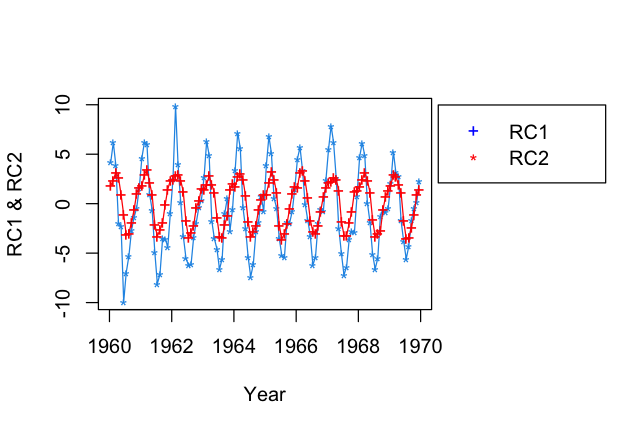
\includegraphics[width=0.98\textwidth]{./gaphics/q002_d.png}
\caption{Timeseries of PCA Rotations} 
\label{fig2}
\end{figure}
Figure 5  describes proportion of variability captured by each Principal  Rotated Components (RC1 and RC2) on the
original data and the component scores.  The scores shows how each process varies in the time domain.  RC1 most active in 2, most inactive in 1968 but was dormant in 1975. There overall trend shows that both principal components periodically have strong influence on the amount of Potential Evapotranspiration of the ten cities.

\begin{figure*}[!h]
    \centering
    \begin{subfigure}[t]{0.5\textwidth}
        \centering
        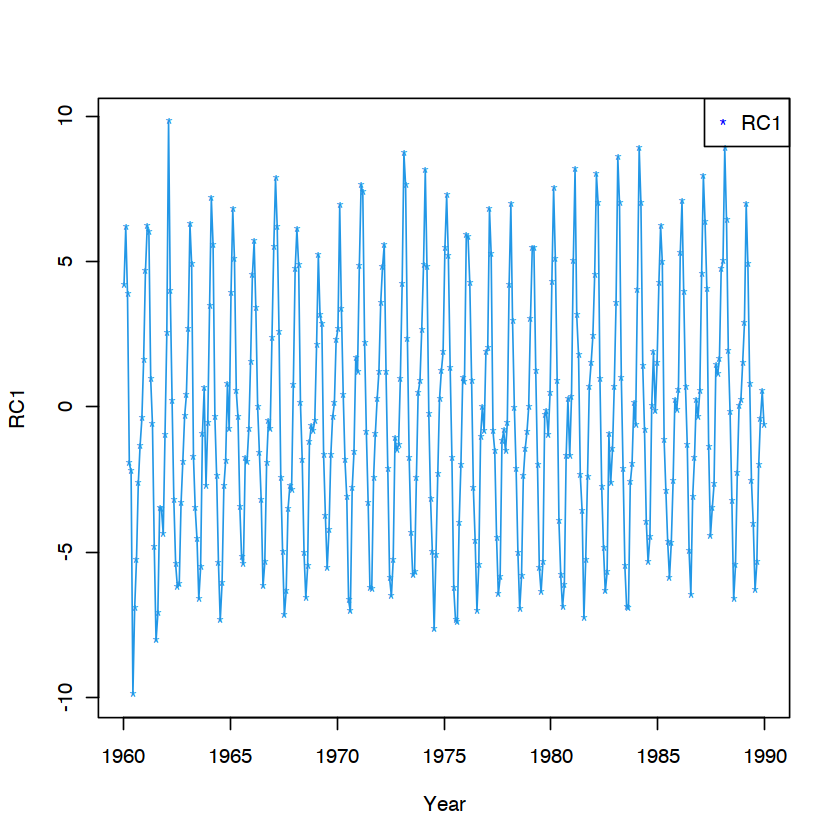
\includegraphics[height=1.9in]{./gaphics/q002_e.png}
        \caption{Timeseries of PCA Rotation 1 and Linear Fit} 
    \end{subfigure}%
    ~ 
    \begin{subfigure}[t]{0.5\textwidth}
        \centering
        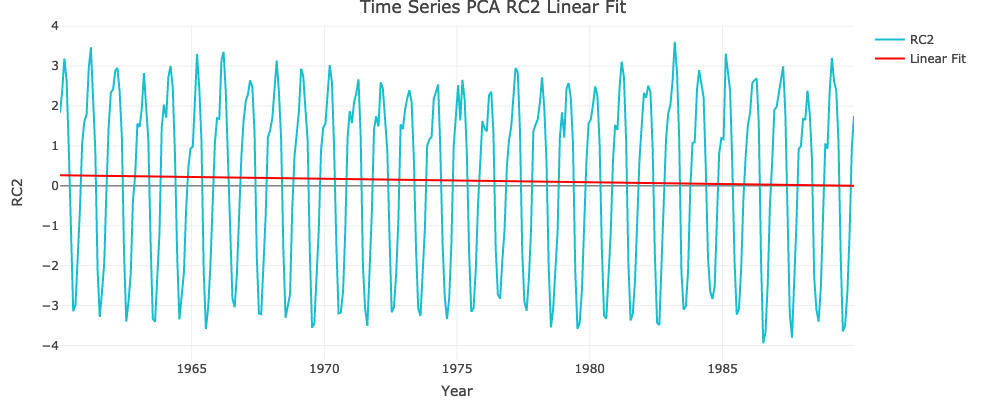
\includegraphics[height=1.9in]{./gaphics/q002_f.png}
        \caption{Timeseries of PCA Rotation 2 and Linear Fit} 
    \end{subfigure}
    \caption{Principal Component Analysis: Linear Fit}
\end{figure*}

\begin{figure*}[!h]
    \centering
    \begin{subfigure}[t]{0.5\textwidth}
        \centering
        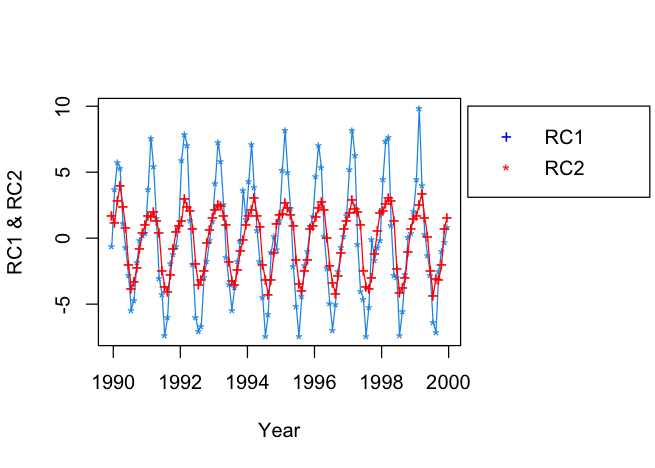
\includegraphics[height=1.9in]{./gaphics/q002_g.png}
        \caption{}
    \end{subfigure}%
    ~ 
    \begin{subfigure}[t]{0.5\textwidth}
        \centering
        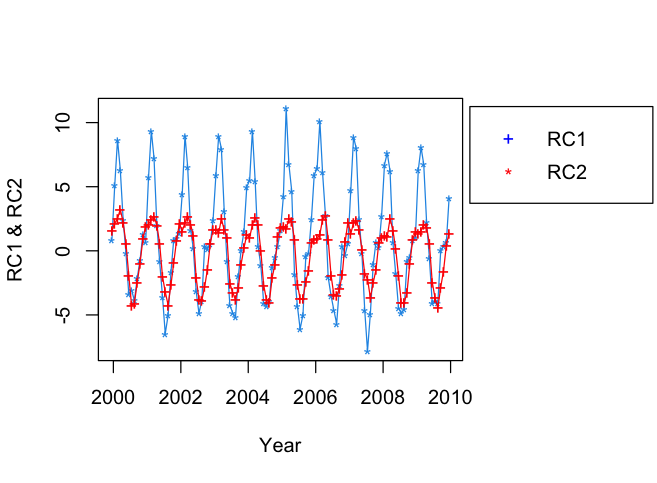
\includegraphics[height=1.9in]{./gaphics/q002_h.png}
        \caption{}
    \end{subfigure}
    \caption{Principal Component Analysis: detrended}
\end{figure*}

\begin{figure*}[!h]
    \centering
    \begin{subfigure}[t]{0.5\textwidth}
        \centering
        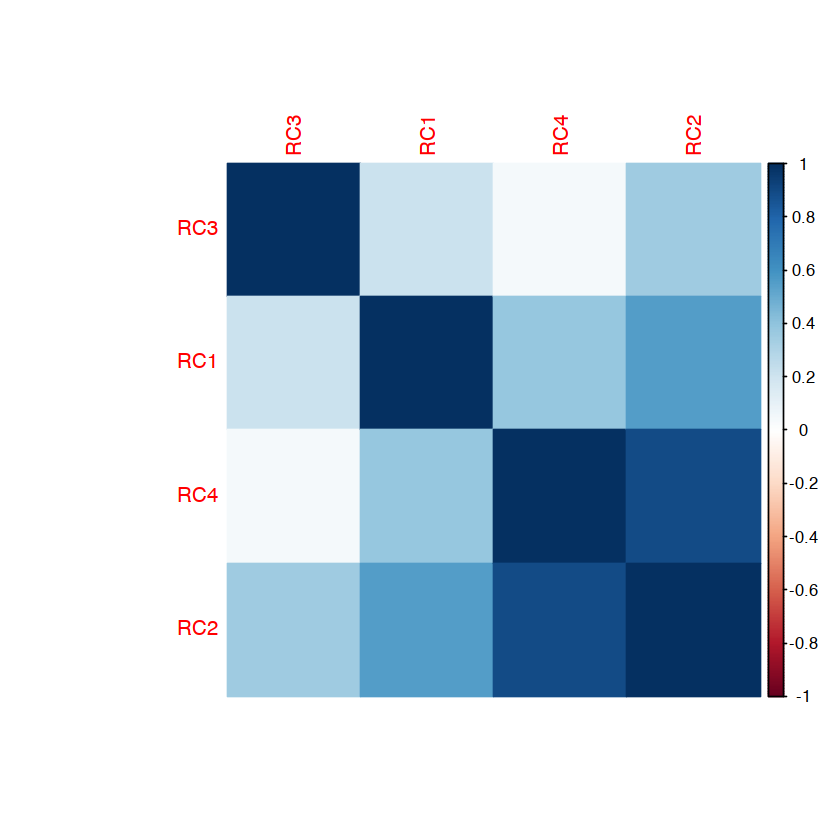
\includegraphics[height=1.9in]{./gaphics/q003_a.png}
        \caption{Rotation Factors}
    \end{subfigure}%
    ~ 
    \begin{subfigure}[t]{0.5\textwidth}
        \centering
        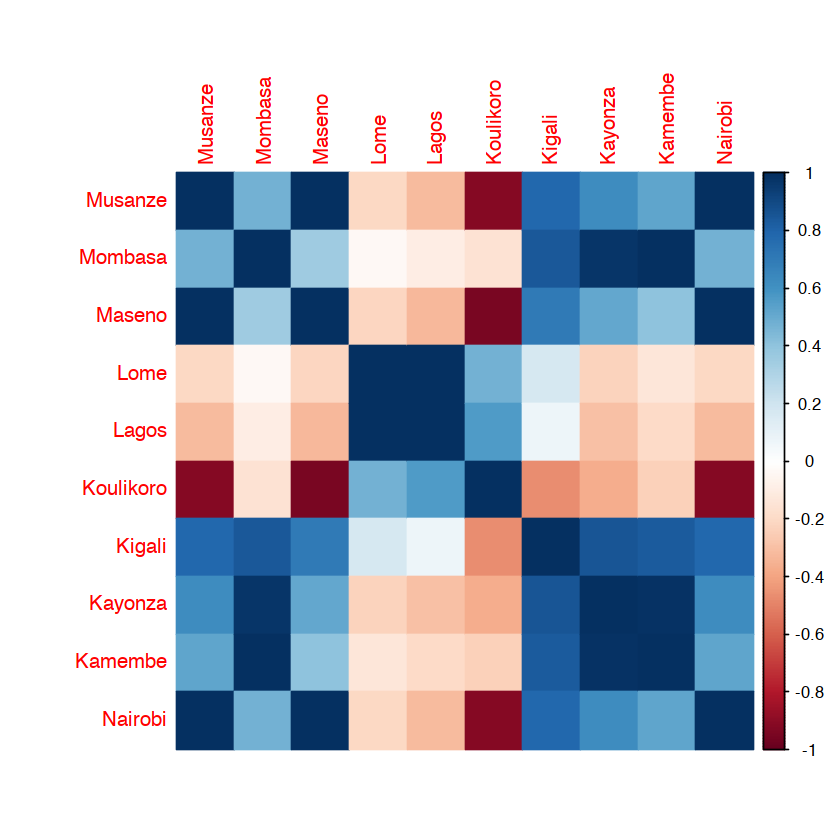
\includegraphics[height=1.9in]{./gaphics/q003_b.png}
        \caption{Cities PET}
    \end{subfigure}
    \caption{Principal Component Analysis: Factor Correlation}
\end{figure*}

\begin{figure}[!h]
                 \centering
                 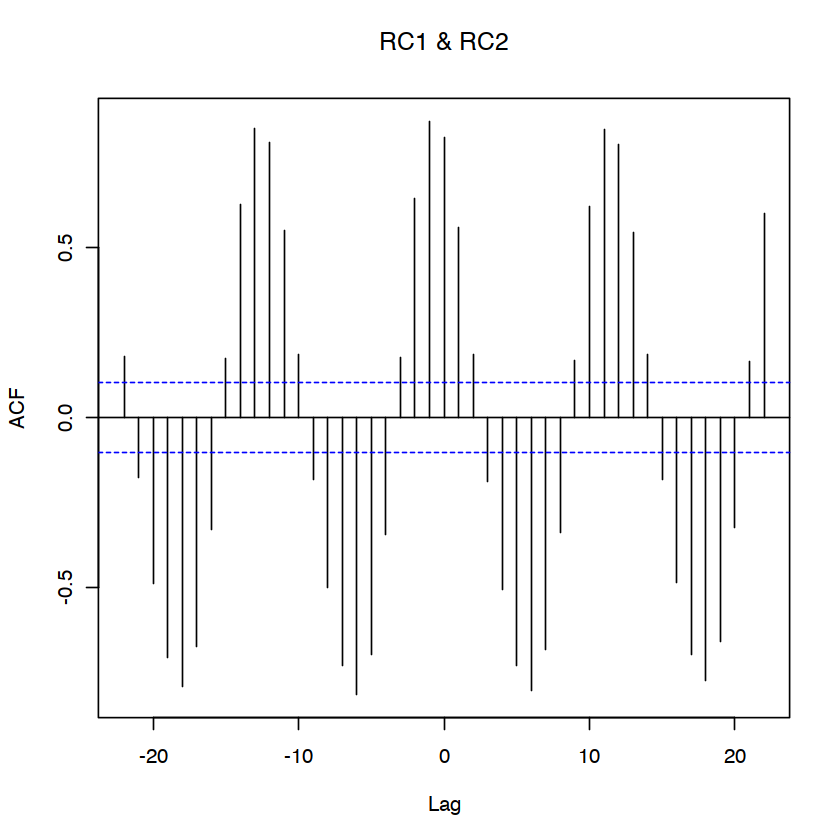
\includegraphics[width=0.98\textwidth,height=180pt]{./gaphics/q003_c.png}
\caption{Timeseries of PCA Rotations: Cross-correlations} 
\label{fig2}
\end{figure}

\begin{figure*}[!h]
    \centering
    \begin{subfigure}[t]{0.5\textwidth}
        \centering
        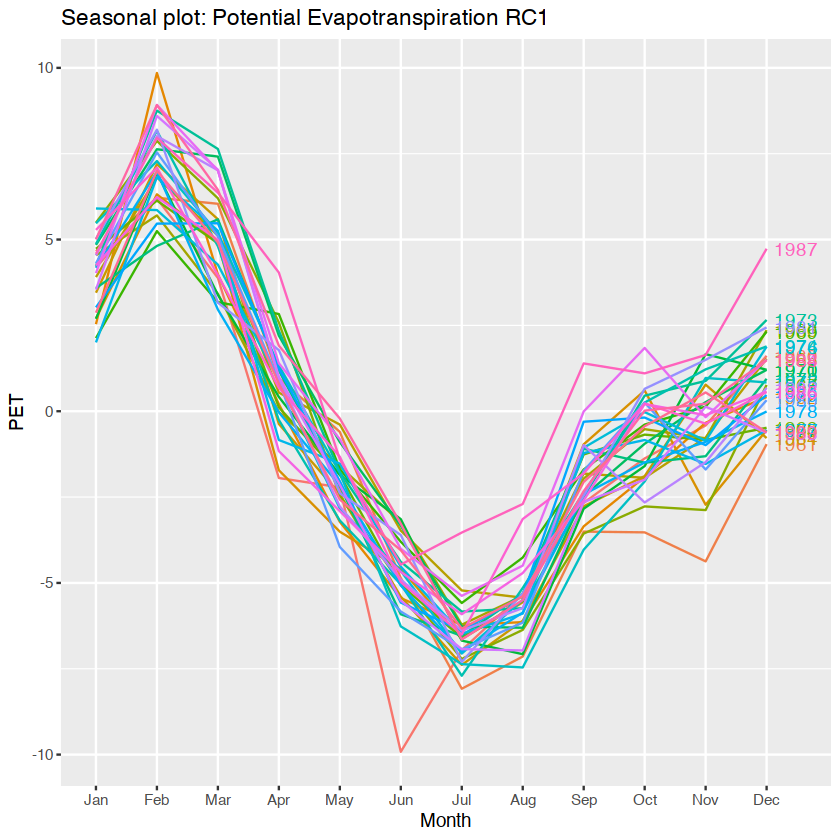
\includegraphics[height=1.9in]{./gaphics/q003_d.png}
        \caption{}
    \end{subfigure}%
    ~ 
    \begin{subfigure}[t]{0.5\textwidth}
        \centering
        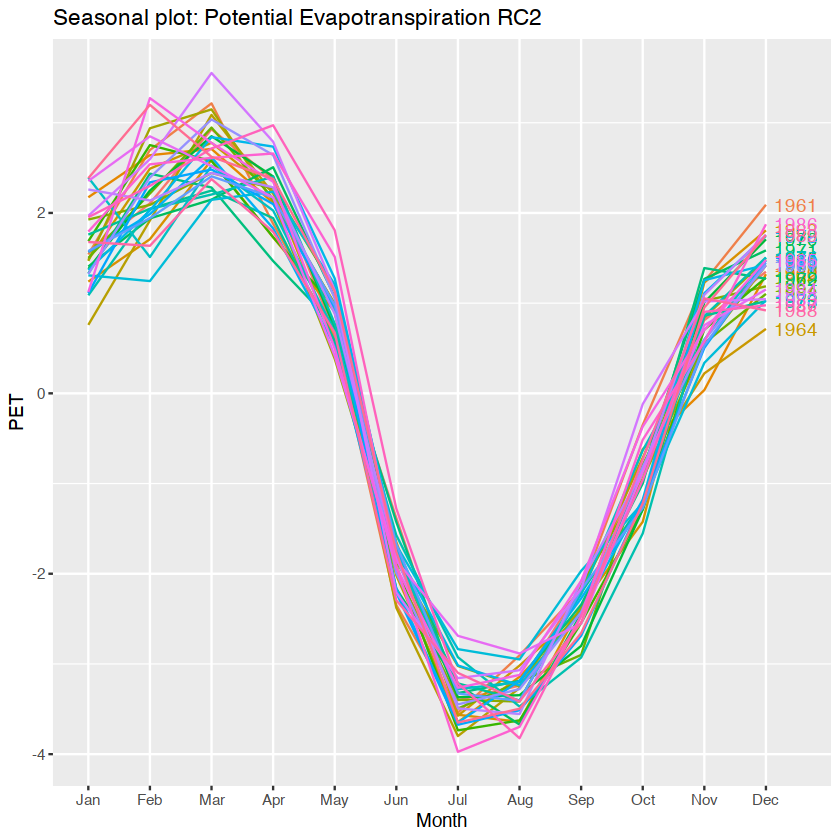
\includegraphics[height=1.9in]{./gaphics/q003_e.png}
        \caption{}
    \end{subfigure}
    \caption{Principal Component Analysis: Scores Periodicity}
\end{figure*}

\begin{figure*}[!h]
    \centering
    \begin{subfigure}[t]{0.5\textwidth}
        \centering
        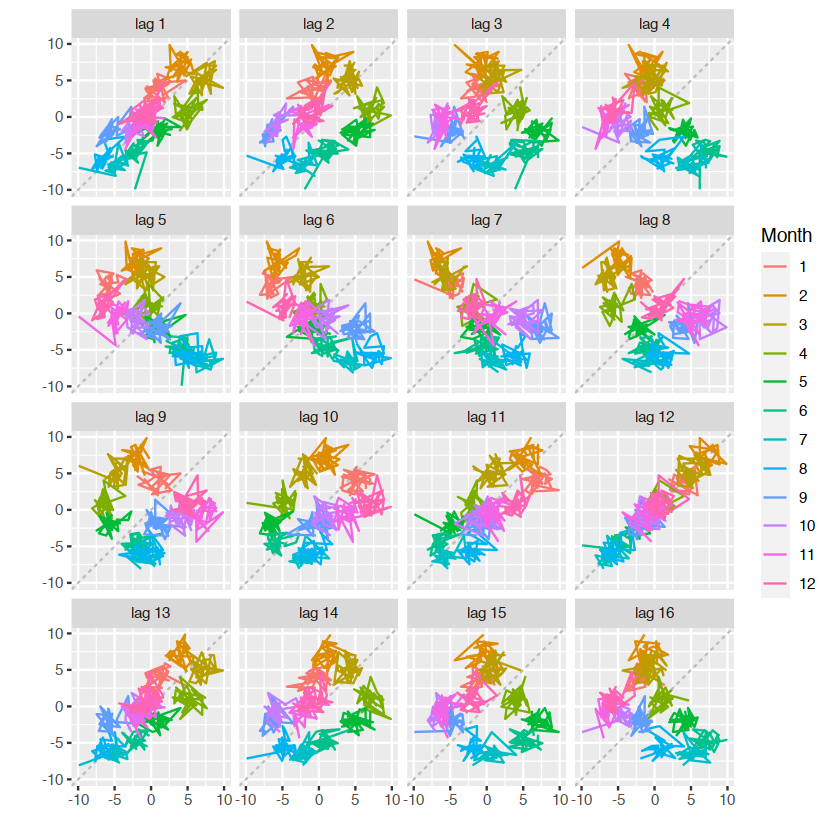
\includegraphics[height=1.9in]{./gaphics/q003_f.png}
        \caption{}
    \end{subfigure}%
    ~ 
    \begin{subfigure}[t]{0.5\textwidth}
        \centering
        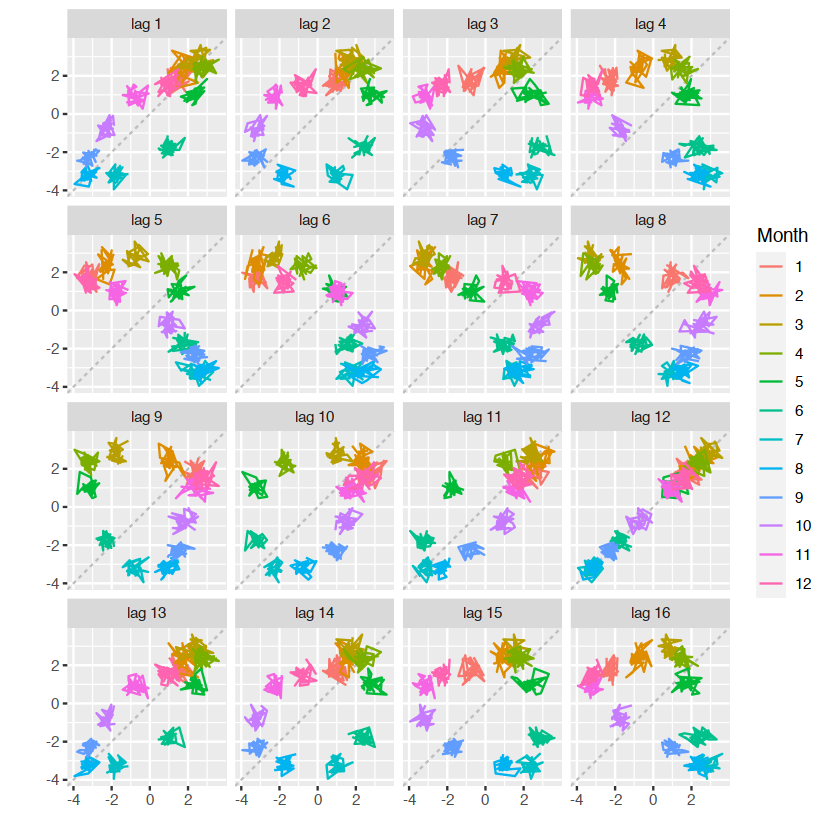
\includegraphics[height=1.9in]{./gaphics/q003_g.png}
        \caption{}
    \end{subfigure}
    \caption{Principal Component Analysis: Lagged Plots}
\end{figure*}

\section{Conclusion}
In this report,  we have explored Potential Evapotranspiration phenomenon across ten geographically different African cities using CA algorithms (using 3 distinct linkage methods) find their PET groupings, and we further,  used PCA to perform dimensionality reduction to identity the underlying processes that generated the data set.   
Using CA,  we identified four distinct PET clusters as shown in  Figure 2(a).
\end{document}